%-------
% Notes
%   ~ADD       : Add the following.
%   ~REFERENCE : Reference the following paper/authors.
%   ~FIND      : Find a paper regarding the following.
%   ~CHECK     : Check that the following is met.
%   ~READ      : Read through the following paper/authors.
%   ~MENTION   : Mention the following.
%   ~AMMEND    : Make a change to the following.
%   ~IDEA      : Suggestion for later in the project.

\documentclass{UoYCSproject}
\usepackage{graphicx} % For images
\graphicspath{ {img/} }

% -----------
% Tikz Setup 
\usepackage{geometry}
\usepackage{tikz}
\usetikzlibrary{ matrix,      % For easy node positioning
                 fit,         % For easily fitting nodes inside another one
                 arrows,
                 positioning, % For easy node-relative placements
                 decorations.pathreplacing,
               }
\tikzstyle{edge} = [->, bend left]
\tikzstyle{biedge} = [bend left]
\tikzstyle{edge'} = [->, bend right]
\tikzstyle{biedge'} = [bend right]
\tikzstyle{edge_str8} = [->]
\tikzstyle{biedge_str8} = []
\tikzstyle{vertex} = [circle, minimum width=0.8cm, text centered, draw=black]
\tikzstyle{mark_red} = [fill=red]
\tikzstyle{mark_violet} = [fill={rgb:red,0.5;blue,0.5;white,1}]
\tikzstyle{mark_grey} = [fill={rgb:black,1;white,3}]
\tikzstyle{graph_small} = [rectangle, draw=black, inner sep=0.5cm]
\tikzstyle{graph} = [rectangle, draw=black, inner sep=1cm]
\tikzstyle{rule} = [rectangle, inner sep=1cm]
\tikzstyle{derivation} = [-implies, double, thick, double distance=1mm, shorten >=6pt, shorten <=6pt]
\tikzstyle{code} = [font=\ttfamily]

% ---------------
% Listings Setup
\usepackage{listings}
\lstset{basicstyle=\footnotesize\ttfamily,breaklines=true}
\usepackage{courier}

\author{Huw Taylor}
\title{Tracing \& Debugging GP2}
\date{\today}
\supervisor{Dr. Detlef Plump}
\MEng
%TODO ~CHECK: The word/page counts are up to date.
\wordcount{10216}
\pagecount{29}
% ~16000 words (55 pages) total
\abstract{
% ~66 words
This project adds tracing of graph programs to the GP2 system. Intermediate steps of a graph program are outputted and these resultant graphs can be viewed like any other. The steps can be specified at runtime and can be as small as a rule match, and as large as the entire graph program. The GP2 compiler has been modified to compile the runtime program to add breakpoints which can be activated upon passing step-count and step-size parameters to the runtime code.
}

\acknowledgements{
I would like to thank Christopher Bak for his continued support throughout the project. His advice on the workings of the GP2 compiler has been invaluable. I would also like to thank Detlef Plump for his help, as well as for his faith in me.
}

\begin{document}
\pagenumbering{gobble}
\maketitle

\tableofcontents

\chapter{Introduction}
\pagenumbering{arabic}
% ~1333 words
\section{Motivation}
GP is a graph programming language. It was developed to provide a language that is expressive enough to solve complex graph problems, while also having a simple enough syntax to allow for formal reasoning. Graphs and graph transformations have previously been implemented in low-level languages, like C. This meant that it was more difficult to understand, verify, and implement \cite{gp_lang}. GP at its core has four commands that nevertheless allows every computable function on graphs to be implemented \cite{gp1}. These commands are a single application of a rule, sequential composition, loops, and branching. Loops are implemented in a run-for-as-long-as-possible style.

GP2, the second iteration of GP, builds upon the first. It adds a few new features, and some syntactic sugar \cite{gp2_design}. Also, the design of GP2 was slightly modified to enable a higher level of performance \citep{chris_compiler}. A compiler was produced by the University of York for GP2. The compiler generates C code from a high level representation of a graph program in GP2. This has the advantage of being able to reason about graphs and graph programming using GP2, but allows for the low-level, high-performance that C allows for \citep{compiling_gp2}.

The University of York has also produced a graphical editor for creating graphs and graph programs. The editor depends on the compiler to execute a given graph program on the host graph, thereby producing the resultant graph. It displays the graphs, and has a graphical user interface for creating graphs, rules and graph programs.

Currently, the compiler generates the code to run the entire graph program on the given host graph. It generates code for each rule and a main graph program file which makes use of the rules' code. After compilation, the C code implementation of the graph program can be run on the graph, and the resultant graph is saved in the given output directory.

If the graphical editor is being used, the user can graphically create the host graph, and the rules for the graph program within it, and can run their program on their host graph, and the editor will show them the resultant graph.

There is no way to debug a graph program for correct behaviour. The compiler will give the user messages regarding incorrect syntax, but a user has no way of debugging an incorrect implementation of a graph program that has correct syntax. This is exacerbated by the fact that the compiler simply outputs the resultant.

The aim of this project is to show the execution of the program, that is, the intermediate steps that result in the final output graph. This will allow users to see the process, which enables the correctness of the program to be ensured. It will also give people using these tools, who may not have a complete understanding of how graph programs work in general, or who aren't sure about their specific program's execution in particular, the opportunity to see the process with a finer granularity.

This tracing of graph programs will sit atop the existing GP2 implementation and be completely optional for any users. It will allow for deeper and more powerful visualisations of graph programs and their execution.
%

\section{Ethics}
The project discussed has very few ethical considerations. It is not related to defence and there are no safety or security concerns. No humans or animals are involved in its development.

\chapter{Literature Review}
% ~4000 words
%~CHECK: Shows that you know what is happening in your field 
%~CHECK: Justifies why your work is interesting or important 
%~CHECK: establishes the theoretical framework/context for your work 
%~CHECK: defends your choice of methodology 
%~CHECK: avoids repeating previous researchers’ mistakes
\section{Graph Programming}

\subsection{Graph Transformations}
A graph is a visual way of representing data and relationships. The formal definition is a set of vertices (nodes) \emph{V}, a set of edges \emph{E}, and a set of labels \emph{L}. Additionally \emph{source} and \emph{target} functions associate edges with nodes, and a \emph{label} function, which assigns labels to edges and nodes.
Graph theory is said to go back as far as the 1730s, with The K{\"o}nigsberg Bridge problem being regarded as the topic for the first paper on graph theory ever written \cite{grathe_origin}. 

The mathematical theory of Graph Transformation allows the transformation of graphs by way of rules. Rules are applied to graphs. They include a LHS (Left-Hand Side) graph, and RHS (Right-Hand Side) graph and an interface graph, which connects nodes in the LHS to nodes in the RHS. There is a convention that if the interface graph is ommited then it is inferred that it comprises the common labelled nodes in both the LHS and RHS.

Rules can either use a single-pushout or a double-pushout approach. In GP, graph transformations use the double-pushout with relabelling \cite[p. 100]{gp1}. Matches of rules must be injective morphisms and are only vaild if they don't result in \emph{dangling edges}, that is, edges with one or more ends not attactched to a node. The interface graph of a rule may be partially labelled, but all other graphs must be totally labelled. A partially labelled graph is a graph with a partial node-labelling function and a total edge-labelling function, whereas a totally labelled graph is where function mapping a label to every node is total.

Figure \ref{fig:simple_rule} shows a simple rule that, given a non-empty host graph, creates a transitive graph, where every node with a directed path to another has a direct edge going to it. A directed path between two nodes \emph{A} and \emph{B} exists either if there is an outgoing edge from \emph{A} to \emph{B}, or for any of the nodes that have an incoming edge from \emph{A}, there is a directed path from it to \emph{B}.
Figure \ref{fig:simple_rule_sans_k} shows the same rule without its interface graph.

\begin{figure}
\label{fig:simple_rule}
\centering
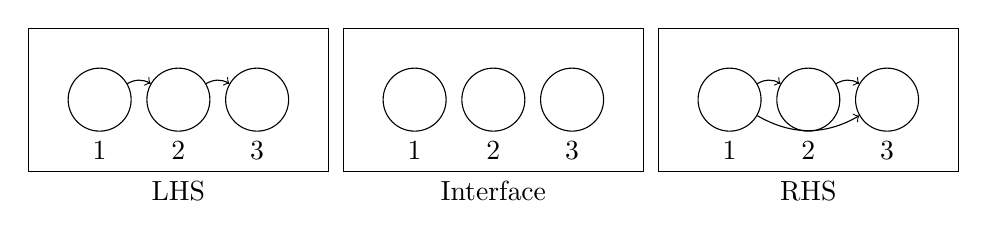
\begin{tikzpicture}[scale=2]
  \node (n1) [vertex, label=below:{1}] at (0, 0) {};
  \node (n2) [vertex, label=below:{2}] at (0.5, 0) {};
  \node (n3) [vertex, label=below:{3}] at (1, 0) {};
  \path [edge] (n1) edge node {} (n2);
  \path [edge] (n2) edge node {} (n3);
  \node (l) [graph_small, fit={(n1) (n2) (n3)}, label=below:{LHS}] {};
  
  \node (n4) [vertex, label=below:{1}] at (2, 0) {};
  \node (n5) [vertex, label=below:{2}] at (2.5, 0) {};
  \node (n6) [vertex, label=below:{3}] at (3, 0) {};
  \node (k) [graph_small, fit={(n4) (n5) (n6)}, label=below:{Interface}] {};
  
  \node (n7) [vertex, label=below:{1}] at (4, 0) {};
  \node (n8) [vertex, label=below:{2}] at (4.5, 0) {};
  \node (n9) [vertex, label=below:{3}] at (5, 0) {};
  \path [edge] (n7) edge node {} (n8);
  \path [edge] (n8) edge node {} (n9);
  \path [edge'] (n7) edge node {} (n9);
  \node (r) [graph_small, fit={(n7) (n8) (n9)}, label=below:{RHS}] {};
\end{tikzpicture}
\caption{Rule Example}
\end{figure}

\begin{figure}
\label{fig:simple_rule_sans_k}
\centering
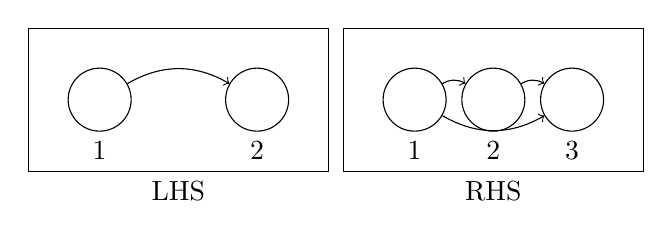
\begin{tikzpicture}[scale=2]
  \node (n1) [vertex, label=below:{1}] at (0, 0) {};
  \node (n2) [vertex, label=below:{2}] at (1, 0) {};
  \path [edge] (n1) edge node {} (n2);
  \node (l) [graph_small, fit={(n1) (n2)}, label=below:{LHS}] {};
  
  \node (n7) [vertex, label=below:{1}] at (2, 0) {};
  \node (n8) [vertex, label=below:{2}] at (2.5, 0) {};
  \node (n9) [vertex, label=below:{3}] at (3, 0) {};
  \path [edge] (n7) edge node {} (n8);
  \path [edge] (n8) edge node {} (n9);
  \path [edge'] (n7) edge node {} (n9);
  \node (r) [graph_small, fit={(n7) (n8) (n9)}, label=below:{RHS}] {};
\end{tikzpicture}
\caption{Rule Example without Interface Graph}
\end{figure}

An application of a rule to a graph will remove the items found in the LHS and not the interface, and then add the items in the RHS not found in the interface, relabelling the nodes that are unlabelled in the interface \cite{gp_lang, gp2_design}. Figure \ref{fig:simple_rule_application} shows the application of the rule shown in figure \ref{fig:simple_rule_sans_k} on a host graph. Step 1 shows the matching of the LHS to the host graph. This match is chosen non-deterministically, and the other possibilities are shown as alternative matches. Step 2 shows the removal of the nodes and edges that are in the LHS and not in the Interface. Step 3 shows the addition of the nodes and edges that are in the RHS and not in the Interface. Step 3 would also be the step to add any labels to nodes, however, the nodes in the host graph and rules have empty labels. The colouring of the nodes is an illustration to draw your attention to the changes as is not a feature of the graph.

\begin{figure}
\label{fig:simple_rule}
\centering
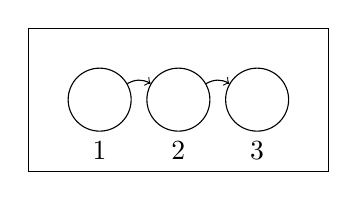
\begin{tikzpicture}[scale=2]
  \node (n1) [vertex, label=below:{1}] at (0, 0) {};
  \node (n2) [vertex, label=below:{2}] at (0.5, 0) {};
  \node (n3) [vertex, label=below:{3}] at (1, 0) {};
  \path [edge] (n1) edge node {} (n2);
  \path [edge] (n2) edge node {} (n3);
  \node (l) [graph_small, fit={(n1) (n2) (n3)}, label=below:{}] {};
\end{tikzpicture}
\caption{Rule Example}
\end{figure}

\subsection{Graph Programs}
The University of York has developed a graph programming language \emph{"GP1"} \cite{gp1}, and has developed a new implementation \emph{"GP2"} \cite{gp2_design}. The goal of both of these has been to write programs that manipulate graphs in terms of the graphs, rather than in general purpose languages like C or Java. 

Graph programming (GP) allows the application of programs to graphs. A program is made up of rules and rudimentary control structures, such as conditions, and loops. The rules are executed non-deterministically on a graph, known as the \emph{host graph}. The resulting graph is known as the \emph{result graph}. A simple program could just be the continued application of a single rule. 

Figure \ref{fig:simple_program} shows an example of a graph program using the GP2 syntax. The first two lines show the program's structure. It shows a procedure 'Traverse', which non-deterministically choses from the rule set containing the rules 'add' and 'reduce'. The main declaration runs the 'init' rule and then runes the 'Traverse' procedure for as long as posisble. The program assumes that the input graph has a single red node, and that none of the edge labels are negative numbers.

The 'add' and 'reduce' rules make use of GP2 addition of marks. Violet matches are the special case whereby they can match any mark.

GP also allows for if-then-else statements, whereby if a condition consisting of a rule set is succesfully applied, the graph \emph{before} the application of the condition has the 'then' branch executed on it. If the condition fails then the else branch is executed, also on the graph before the application of the condition. GP2 adds a try-then-else statement, which acts the same for the else branch, however on a successful application of the condition, the 'then' branch executes on the result of the condition.

The table \ref{table:gp2_ast}, taken from \cite{chris_compiler}, shows the abstract syntax for GP2 programs. It doesn't include the syntax for rule and procedure identifiers, which are strings of alphanumeric characters, starting with a letter. Procedures must begin with an upper-case letter, and rules with a lower-case letter. Also, procedures cannot be recursive, and so by extension cannot call a procedure that calls itself \cite{chris_compiler}. Procedures can be thought of as similar to macros in other languages such as C, that is, its command sequence can be put inline in the place of the procedure with no change in the program.

\begin{table}
\begin{tabular}{l l l}
Prog        & ::= & Decl \{ Decl \} \\
Decl        & ::= & MainDecl | ProcDecl | RuleDecl \\
MainDecl    & ::= & \texttt{main} '=' ComSeq \\
ProcDecl    & ::= & ProcId '=' [ LocalDecl ] ComSeq \\
LocalDecl   & ::= & ( RuleDecl | ProcDecl ) \{ LocalDecl \} \\
ComSeq      & ::= & Com \{ ';' Com \} \\
Com         & ::= & RuleSetCall | ProcCall \\
            &     & | \texttt{if} ComSeq \texttt{then} ComSeq [\texttt{else} ComSeq] \\
            &     & | \texttt{try} ComSeq \texttt{then} ComSeq [\texttt{else} ComSeq] \\
            &     & | ComSeq '!' \\
            &     & | ComSeq \texttt{or} ComSeq \\
            &     & | '(' ComSeq ')' \\
            &     & | \texttt{break} | \texttt{skip} | \texttt{fail} \\
RuleSetCall & ::= & RuleId | '\{' [ RuleId \{ ',' RuleId \} ] '\}' \\
ProcCall    & ::= & ProcId \\
\end{tabular}
\caption{Abstract Syntax Tree for a GP2 program}
\label{table:gp2_ast}
\end{table}

\begin{figure}
\label{fig:simple_program}
\centering
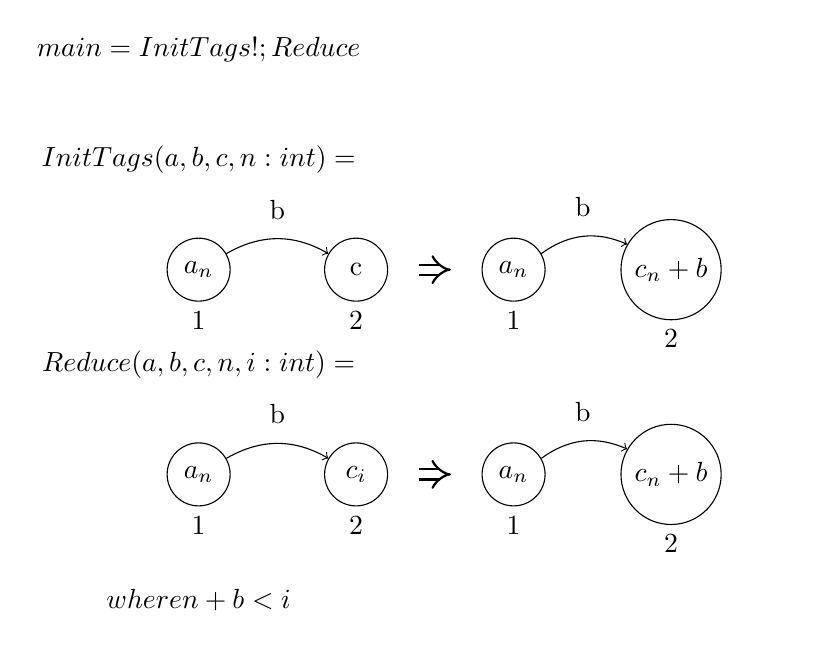
\begin{tikzpicture}[scale=2]
  \node (code) at (0, 3.5) {$main = InitTags!; Reduce$};
  \node (rule_1) at (0, 2.8) {$InitTags(a,b,c,n : int) = $};

  \node (n1) [vertex, label=below:{1}] at (0, 2.1) {$a_n$};
  \node (n2) [vertex, label=below:{2}] at (1, 2.1) {c};
  \path [edge] (n1) edge node[label=above:{b}] {} (n2);
  \node (r1_l) [rule, fit={(n1) (n2)}] {};
  
  \node (n3) [vertex, label=below:{1}] at (2, 2.1) {$a_n$};
  \node (n4) [vertex, label=below:{2}] at (3, 2.1) {$c_n+b$};
  \path [edge] (n3) edge node[label=above:{b}] {} (n4);
  \node (r1_r) [rule, fit={(n3) (n4)}] {};
  
  \draw[derivation] (r1_r) -> (r1_l); % dafuq is this backwards bullshit?
  
  \node (rule_2) at (0, 1.5) {$Reduce(a,b,c,n,i : int) = $};  
  
  \node (n5) [vertex, label=below:{1}] at (0, 0.8) {$a_n$};
  \node (n6) [vertex, label=below:{2}] at (1, 0.8) {$c_i$};
  \path [edge] (n5) edge node[label=above:{b}] {} (n6);
  \node (r2_l) [rule, fit={(n5) (n6)}] {};
  
  \node (n7) [vertex, label=below:{1}] at (2, 0.8) {$a_n$};
  \node (n8) [vertex, label=below:{2}] at (3, 0.8) {$c_n+b$};
  \path [edge] (n7) edge node[label=above:{b}] {} (n8);
  \node (r2_r) [rule, fit={(n7) (n8)}] {};
  
  \draw[derivation] (r2_r) -> (r2_l); % ~EDIT: Maybe use the deriviation tikz thing defined at the top.
  \node (rule_2_condition) at (0, 0) {$where n+b < i$};  

\end{tikzpicture}
\caption{Simple Dijkstra Program Example}
\end{figure}

The program \ref{fig:simple_program} finds the shortest path to each node, using Dijkstra's algorithm for pathfinding. The procedure 'Traverse' isn't strictly necessary - it could be replaced with '\texttt{\{add, reduce\}}', but it serves to illustrate the syntax for procedures. 

Running this program on the host graph shown will give the intermediary graphs shown in figure \ref{fig:simple_program_example_1}. Since GP is non-deteministic, the figure shows only one of the many possible outcomes of applying this graph program. The host graph is making use of another addition of GP2. The undirected edges are syntactic sugar for two directional edges, one going in each direction.

\newgeometry{left=1cm,bottom=0.1cm}

\begin{figure}
\label{fig:simple_program_example}
\centering
%TODO ~CHECK: Make sure this displays how it should.
%TODO ~ADD: Colour to illustrate changes?
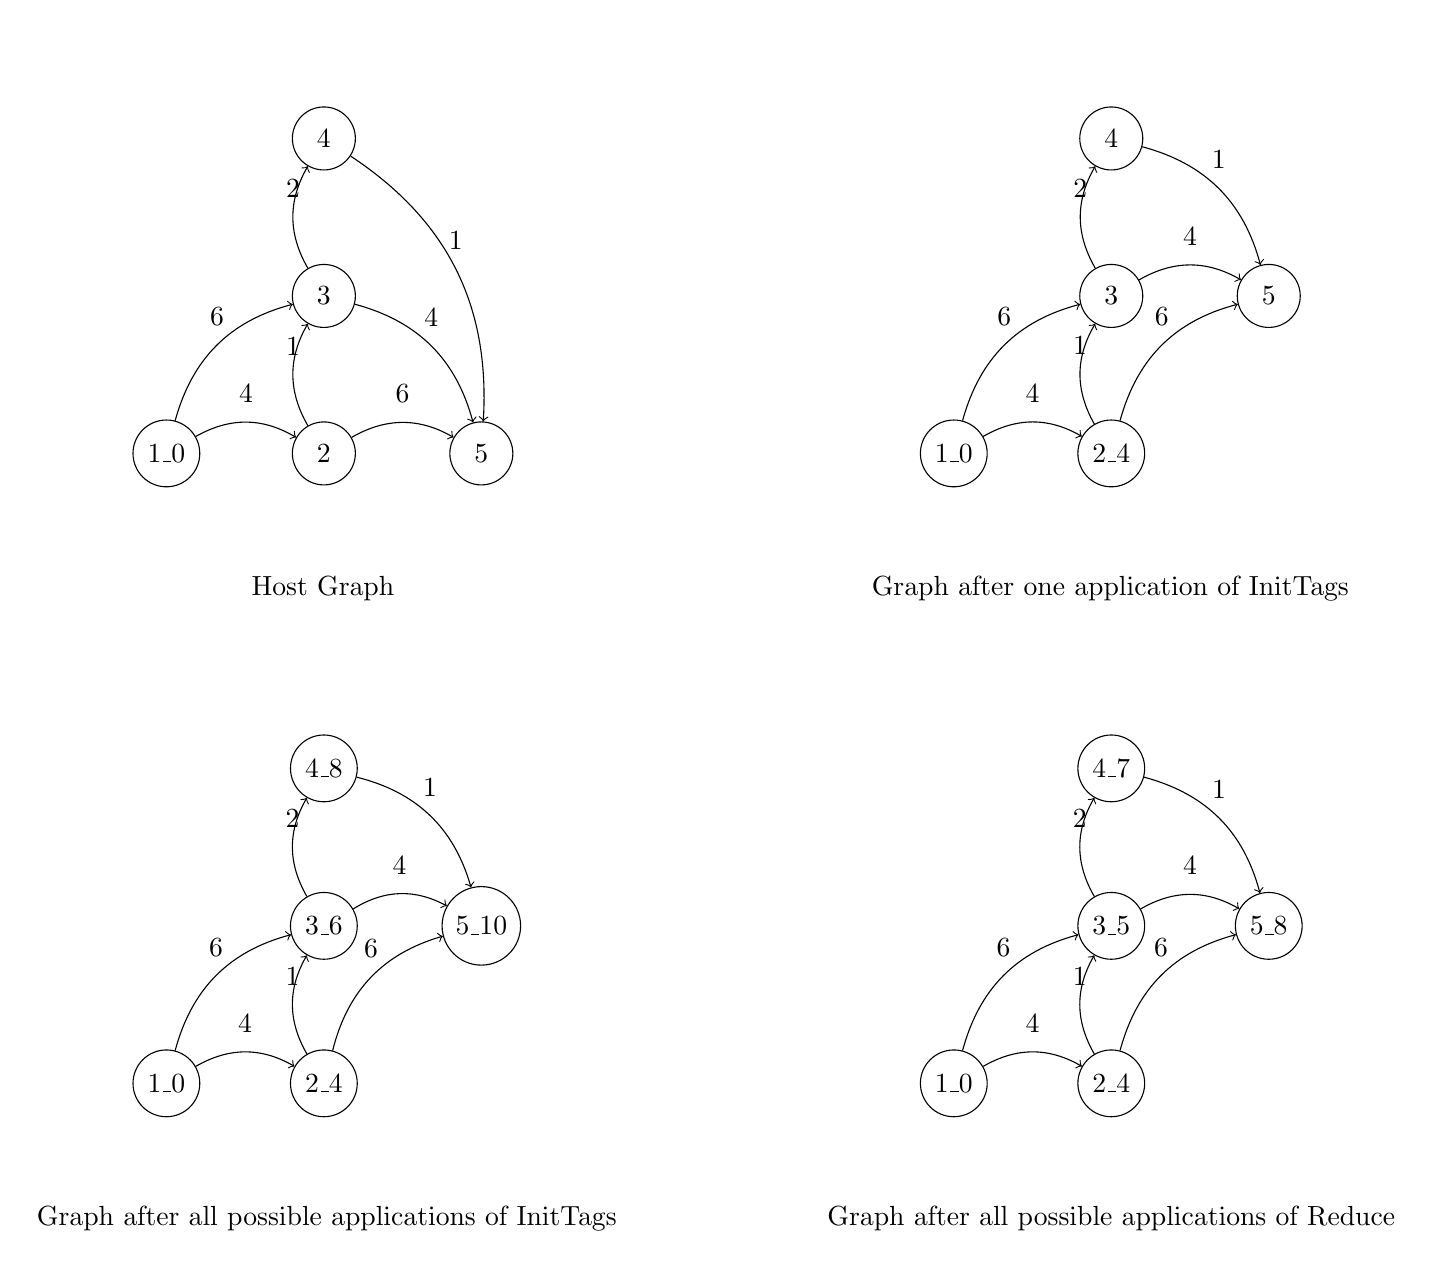
\begin{tikzpicture}[scale=2]
  \node (n1_1) [vertex] at (0, 4) {$1\_0$};
  \node (n1_2) [vertex] at (1, 4) {2};
  \node (n1_3) [vertex] at (1, 5) {3};
  \node (n1_4) [vertex] at (1, 6) {4};
  \node (n1_5) [vertex] at (2, 4) {5};
  \path [edge] (n1_1) edge node[label=above:{4}] {} (n1_2);
  \path [edge] (n1_1) edge node[label=above:{6}] {} (n1_3);
  \path [edge] (n1_2) edge node[label=above:{1}] {} (n1_3);
  \path [edge] (n1_3) edge node[label=above:{2}] {} (n1_4);
  \path [edge] (n1_2) edge node[label=above:{6}] {} (n1_5);
  \path [edge] (n1_3) edge node[label=above:{4}] {} (n1_5);
  \path [edge] (n1_4) edge node[label=above:{1}] {} (n1_5);
  \node (g0) [rule, fit={(n1_1) (n1_2) (n1_3) (n1_4) (n1_5)}, label=below:{Host Graph}] {};
  
  \node (n2_1) [vertex] at (5, 4) {$1\_0$}; % probably have to change these coordinates.
  \node (n2_2) [vertex] at (6, 4) {$2\_4$};
  \node (n2_3) [vertex] at (6, 5) {3};
  \node (n2_4) [vertex] at (6, 6) {4};
  \node (n2_5) [vertex] at (7, 5) {5};
  \path [edge] (n2_1) edge node[label=above:{4}] {} (n2_2);
  \path [edge] (n2_1) edge node[label=above:{6}] {} (n2_3);
  \path [edge] (n2_2) edge node[label=above:{1}] {} (n2_3);
  \path [edge] (n2_3) edge node[label=above:{2}] {} (n2_4);
  \path [edge] (n2_2) edge node[label=above:{6}] {} (n2_5);
  \path [edge] (n2_3) edge node[label=above:{4}] {} (n2_5);
  \path [edge] (n2_4) edge node[label=above:{1}] {} (n2_5);
  \node (g1) [rule, fit={(n2_1) (n2_2) (n2_3) (n2_4) (n2_5)}, label=below:{Graph after one application of InitTags}] {};
  
  \node (n3_1) [vertex] at (0, 0) {$1\_0$}; % probably have to change these coordinates.
  \node (n3_2) [vertex] at (1, 0) {$2\_4$};
  \node (n3_3) [vertex] at (1, 1) {$3\_6$};
  \node (n3_4) [vertex] at (1, 2) {$4\_8$};
  \node (n3_5) [vertex] at (2, 1) {$5\_10$};
  \path [edge] (n3_1) edge node[label=above:{4}] {} (n3_2);
  \path [edge] (n3_1) edge node[label=above:{6}] {} (n3_3);
  \path [edge] (n3_2) edge node[label=above:{1}] {} (n3_3);
  \path [edge] (n3_3) edge node[label=above:{2}] {} (n3_4);
  \path [edge] (n3_2) edge node[label=above:{6}] {} (n3_5);
  \path [edge] (n3_3) edge node[label=above:{4}] {} (n3_5);
  \path [edge] (n3_4) edge node[label=above:{1}] {} (n3_5);
  \node (gx) [rule, fit={(n3_1) (n3_2) (n3_3) (n3_4) (n3_5)}, label=below:{Graph after all possible applications of InitTags}] {}; 
  
  \node (n4_1) [vertex] at (5, 0) {$1\_0$}; % probably have to change these coordinates.
  \node (n4_2) [vertex] at (6, 0) {$2\_4$};
  \node (n4_3) [vertex] at (6, 1) {$3\_5$};
  \node (n4_4) [vertex] at (6, 2) {$4\_7$};
  \node (n4_5) [vertex] at (7, 1) {$5\_8$};
  \path [edge] (n4_1) edge node[label=above:{4}] {} (n4_2);
  \path [edge] (n4_1) edge node[label=above:{6}] {} (n4_3);
  \path [edge] (n4_2) edge node[label=above:{1}] {} (n4_3);
  \path [edge] (n4_3) edge node[label=above:{2}] {} (n4_4);
  \path [edge] (n4_2) edge node[label=above:{6}] {} (n4_5);
  \path [edge] (n4_3) edge node[label=above:{4}] {} (n4_5);
  \path [edge] (n4_4) edge node[label=above:{1}] {} (n4_5);
  \node (gn) [rule, fit={(n4_1) (n4_2) (n4_3) (n4_4) (n4_5)}, label=below:{Graph after all possible applications of Reduce}] {}; 
  
\end{tikzpicture}
\caption{Simple Dijkstra Program Example}
\end{figure}

\restoregeometry

\section{GP2 Compiler}
Instead of using an abstract machine as GP1 did, the GP2 compiler generates C code directly \cite{chris_compiler}, which removes the reliance on specific abstract machine compilers and data formats for graphs and graph programs. It means that any C compiler can be used to generate the program code. It also attempts to standardise and document the format of graphs and programs that it takes. This means that tools to generate graphs either graphically or programmatically can be created without reducing modularity or creating complexity and interdependance between the components of the system \cite{gp2_ide}.

GP2 adds to GP the marking of nodes with a colour, or a special 'any' colour; additional conditions that can be checked against in a rule's schema, including the in-degree and out-degree of an edge, and whether there exists an edge between two nodes; and an additional branching mechanism: a try-then-else. In try-then-else and if-then-else branching, the condition is a set of rules schemata, and almost always alters the graph. If-then-else branching uses the graph before the 'if' condition is evaluated, and any changes are made, in the 'then' branch. In contrast, the try-then-else uses the \emph{result} of the 'try' condition in the 'then' branch. In both, the 'else' branch uses the graph before the condition is checked against \cite{gp2_design}.

GP2 no longer enforces non-deterministic execution \cite[p. 15]{gp2_ide}, and doesn't backtrack to reach all possible solutions. This was done to achieve a higher level of implementation efficiency \cite[p. 15]{chris_compiler}, but sacrifices completeness. Backtracking is still employed, but only in if and try statements and in loop bodies, but GP2 doesn't ensure that all possible results of a graph program on a host graph are returned \cite[p. 65]{chris_compiler}.

The GP2 compiler parses the program and host graph files, and generates a C code representation of the program, which can then be run. It generates an abstract syntax tree for the program, and creates files for each rule, with methods for matching, and methods for applying. These files, along with the main file are stored in a specified output directory, or in \texttt{/tmp/} if none is given. The compiler hard-codes the location of the host graph into the generated runtime program \citep{chris_compiler, compiling_gp2}.

\section{GP2 Editor}
The GP2 graphical editor for creating graphs and graph programs is currently under development. It will allow for the creation of graphs graphically, rather than textually, and it will allow for the creation of programs textually, and their rules graphically, assigning the LHS and RHS of the rules. In contrast with the GP1 editor, the GP2 editor will also include functionality to display nodes and edges in accordance with their marks. It has several tabs. The first simply contains a welcome message for the user, but the 'Edit' tab allows for the user to create and edit graphs, rules and programs. The 'Run' tab simply allows the user to choose a host graph and a graph program and runs the program on the graph. The 'Results' tab shows the resultant graph.

\begin{figure}
\label{img:editor_graph}
\includegraphics[width=\textwidth]{editor_graph}
\caption{The GP2 Editor's Edit Graph View}
\end{figure}

Figure \ref{img:editor_graph} shows the graph editor. It allows users to create nodes and edges, and edit their labels and marks. It can open graph files, but only if they have the correct filetype (\texttt{.host}). You can navigate through large graphs by zooming and panning.

\begin{figure}
\label{img:editor_rule}
\includegraphics[width=\textwidth]{editor_rule}
\caption{The GP2 Editor's Edit Rule View}
\end{figure}

Figure \ref{img:editor_rule} shows the rule editor. It has two small panes that function similar to the graph editor, and has a textbox for rule conditions. Rules can currently not be removed from a project.

\begin{figure}
\label{img:editor_program}
\includegraphics[width=\textwidth]{editor_program}
\caption{The GP2 Editor's Edit Program View}
\end{figure}

Figure \ref{img:editor_program} shows the program editor. It is a simple text editor featuring syntax highlighting.

\begin{figure}
\label{img:editor_result}
\includegraphics[width=\textwidth]{editor_result}
\caption{The GP2 Editor's Results Tab}
\end{figure}

Figure \ref{img:editor_result} shows the resultant graph. You can navigate it by zooming and panning in the same way as the graph editor.

The editor reads the positions of nodes from the graph's file. Positions were added to the GP2 lexer for this very purpose, and the parser simply ignores them. This allows the editor to maintain structural consistency with the graphs. This is a simple technique that is appropriate for this purpose, but cannot be overused, as this would severly complicate the lexing of GP2 programs and graphs.

\section{Program Tracing}
There are several techniques available to software developers when attempting to track down the locations of errors they've made. This process is called debugging, and many of the techniques involve outputting information about the program and its state throughout its execution. Other techniques involve dumping the last-stable memory at the point of a program crashing, which will then be analysed. 

Just-in-time (JIT) Compilers compile code on-demand while the program is being executed. This technique employs the use of detecting start and end points in the code between and compiling between them. Traditionally the unit of a method is used, however loops have also been used as a unit of compliation \cite{jit_trace}.

\subsection{Tracing}
Tracing through the steps of a program has been around since programs themselves. The BASIC programming language had a command \emph{TRON}, short for TRace ON, which print the line numbers of each command as the program ran. 
Tracing allows programmers to ensure that each step is procuding the right results and allows a more detailed insight into the workings of a program. This is done by logging information about the execution of a program that will be useful for debugging or diagnostics, formal methods of which have been discussed as far back as the 70s \cite{psych_debug, code_walkthroughs}.

Although tracing, when as simple as possible, can be merely the addition of a few print statements, when applied throughout a program as a debugging tool, because tracing is generally such a low-level process, there's potential for a vast amount of logging messages \cite{tracing_book}, which can impact performance. Usually programs have either run-time or compile-time options for turning off debugging to combat this.

The trace is also usually only seen by the developer of a system, and so there is no need to have the messages be readable by, or understandable to, the users. This means it can be cheap to implement. However, due to the fact that tracing is a cross-cutting concern \cite{wiki_tracing}, meaning that is is involved all throughout the program, it's difficult to decouple and modularise.

The points within the program where information is divulged are referred to as tracepoints. They are hooking mechanisms which allow for tracing with little overhead when disabled, but that can be enabled at run-time and will provide static tracing \cite{tracing_book}.

\subsection{Breakpoints}
Breakpoints allow for the stopping or pausing of a program part of the way through its execution. This is done to allow usually to obtain knowledge about the state of the program at certain points throughout the process. \emph{Instruction Breakpoints} interrupt the program before an instruction is executed, but there are also \emph{Conditional Breakpoints}, or \emph{Watchpoints}, which trigger upon events such as reading from, or writing to, specific memory locations, or upon certain keystrokes.

\chapter{Design}
\section{Users \& Requirements}
% ~2000 words (Problem analysis)
% ~3333 words (between Design *and* Implementation)

The users of GP2 as it stands are predominantly students and staff at the University of York, and researchers in the field of graph transformations. The students use it to get a hands-on appreciation of both graph transformation generally, and GP2 specifically. The key quality attributes regarding all users will be usability. The tracing of GP2 should serve to increase usability. 

Another stakeholder in the system that isn't a user is future developers, adding to, and maintaing, the software. The quality attributes that are most relevant to these stakeholders are maintainability and integratability. Therefore any additions made must keep these factors in mind.

Any tracing will need to not have any negative impacts on the currently existing system. Ideally, as little effect on efficiency and performace as possible should be made to the compiler, and to the generated code running the Graph Program. And as little effect on usability should be made with regards to the editor. The new system should also be completely backwards compatible. That is, the tracing should be optional, with the current implementation for running a given graph program on a host graph still performing that action.

Also, any changes made to the editor should serve only to enhance the user's understanding of the underlying process, and should be avoidable if they so choose.

It is critical to correctly identify the requirements for a system to be determined successful to allow for any evaluation. It also means that throughout the design process, there are key features to be kept in mind.
\begin{enumerate}
	\item A program must be able to be stepped through, that is, a portion of the program (step) must be able to be run on either the host graph, or the resultant graph of a previous step's execution.
	\item These steps would ideally be of specifiable sizes.
	\item These steps must be able to be displayed graphically in the GP2 Editor.
	\item The changes to the graph made during these steps are to be made available.
	\item These steps would ideally be displayed in such a way to highlight any changes made in a step.
\end{enumerate}

\section{High-Level Design}
Writing maintainable code involves ensuring that the intent behind each procedure is as clear as possible to a programmer, familiar or unfamiliar with the system. This can be done with clear and useful naming of variables and functions, and with appropriate levels of comments documenting the intent behind the code.

A possible design that meets the first aims of this project would be to have the compiler generate "chunks" of the program. This would have shifted most of the extra processing into the compiler, and so would have had minimal impact on the running of the graph program. This could also allow for a greater level of modularisation, with the system potentially being able to assess these chunks independently.
However, this presents the problem that the compiler doesn't know the execution of the program at compile time, and so the sizes of these "chunks" cannot be determined. This means that the smallest size of chunk would have to be generated, and the runtime would determine how many of these correspond to a larger size of step. This also has the problem that the runtime needs to keep track of the current iteration of a loop, which is because the compiler doesn't know how many iterations of a loop will be run at compile time, so it cannot generate the program as a series of steps as it will be run. While this process doesn't have a significant impact on performance if the user is just performing a single step at a time, if the entire program is run, which is the default behaviour, there is a significant performance hit. If a large number of steps is needed to be run, then that requires the program to read in each chunk of code and execute it, for every step. Clever implementations could cache the loaded data, but this sort of file I/O is less costly if just performed once at the beginning.

This design also radically changes the structure of the existing compiler, and changes the flow of executing a graph program. For maintainability, the decision was made against changing the compiler in such a drastic a manner.

An alternative approach is to keep the compiler as it is, but to have it also generate breakpoints in the program code. These breakpoints would allow the program to end after a certain number of steps. Following this, program also needs to be able to start from a step other than the beginning so a user can step through more than once consecutively. This simpler design has less impact on the flow and structure of the compiler as it is, and should have very little impact on the runtime performance of the graph program if the user is executing the entire program. This is an improvement over the previous design in the case where the user is not stepping through the program at all. In the case where the user \emph{is} stepping through, the time taken to get the program state ready to perform the next step(s) is simply the time for a counter to reach the number n, where n is the last executed step. It doesn't need to perform any of the rule matches or applications, it's just traversing the runtime code's structure counting up to the current step. 

This approach obviously needs some way of keeping track of the last executed step, but it also has another problem to solve. Since GP is still non-deterministic, a method is needed to make sure the current step is correctly obtained. This method will need to ensure that each of the decisions chosen from rule sets and if- and try-statement branches is the same for each subsequent step through the program, until the program has terminated. This method could employ a lookup table of the decisions. This lookup table, along with the last executed step, could be stored in a small file alongside the output graph. Loading and saving to this file should have very little impact, and creating the lookup table when executing the graph program is also a simple process.

Since the smallest steps of any relevance to the user are the matching and applications of a rule, this could be the smallest size of step. However, since only the match step of the last rule being run matters at all to the user for the tracing, the decision to have a single rule application as the smallest step makes more sense. This doesn't solve the issue of the user being able to stop between a match and a step, but a simple flag to stop after a match, and before an application, of a rule would be a simple solution. However, this could be presented to a user as a step size for consistency.

A problem arises when the user has stepped through rule applications to the point where the current step is some part of the way through a procedure, and then specifies to step through a number of procedures. Since not all procedures are of the same length, running to "the same point" in subsequent procedures is meaningless, so either the first procedure step must be finishing the current procedure, or this must be done before procedure steps are begun to be counted. This can be generalised to all larger step sizes than have previously been run. The former choice, that of finishing the current step size as the first step of that size, makes sense when considering that running the program (the largest possible step size) from some way through the program, would obviously not finish the 'program' step and then run the program again.

Once stepping through the program is working, the resultant graph has to be saved somewhere for the editor to display it. This intermediate graph can either have its own file, or be saved as the output graph of the program. Having its own file may allow for further applications beyond this project, but being saved in the place of the resultant graph doesn't disrupt the existing flow of the overall system. The decision was made to use the latter, because it is a simple change for any future developer, and it has the least impact on the current system.

The last problem to solve is that of illustrating what changes have happened. It's possible a user is able to visually see new nodes and edges after a rule application, but in a large graph this may be more difficult. 

New nodes and edges are not the only changes that are to be "highlighted". Matched nodes and edges are also to be shown to the user, as well as relabelled nodes and edges. Removals cannot be shown as there is nothing to show, and nothing to attach a "highlight" to.

It's possible to have another file that would list each node and edge that has been added (or matched). This has the advantage of simplicity, but whereas the file containing the current step and branches is only accessed by the runtime code, any file containing the changes made in the last step would be accessed by the graphical editor, and potentially other applications further down the line. Therefore it seems more acceptable to have a more formal way to have this information be accessed. The idea of adding a specific label string for certain changes to a node's label was considered, but this would break functionality of GP2, as any conditions checking for a node's label to be empty would be invalidated by the existance of this 'change label'.

The current implementation of the GP2 Editor adds positions for nodes to the GP2 lexer. They are used by the editor to maintain structure of a graph and keep nodes in the same place where possible. They are used soley by the editor and the parser is instructed to ignore them. Since any "highlight" of a node is a similar type of information, that is, it pertains to not to the mathematical structure of the graph, but is useful in displaying it, it seems appropriate to use this approach for storing the changes of nodes.

\section{Design Breakdown}

Having identified key design problems and thought about preferred solutions, a breakdown of the proposed design is presented. There are certain things the compiler now needs to know in order to process tracing. The first of these is whether to do it at all. Given that the number of steps to perform and the size of those steps are to be passed to the program, the existence of these parameters are enough for the program to decide that it should perform tracing. These parameters also could require each other, as the size of the step is useless without how many of these steps are to be performed, and the number of steps is useless without knowing the size of the step. Alternatively there could be default values for these parameters. 

A default value for step size could either be a rule application, or a match/application of a rule, as these are the smallest step sizes. Any decision between these would be arbitrary and easy to change. A default value should be, for usability reasons, the value that is most often used. The tracing system being implemented here will use a rule application as its default step size, but ideally this would be reassessed when data of the size of steps users are most likely to run is obtained.

A default number of steps is less intuitive, as the program by default will run all the steps, however if tracing is being used by the user, perhaps a default value of a single step of the specified size could be used. 

The program needs no further information from the user to trace through steps, but requires information regarding the last executed step, if there was one. If not, then the program is simply starting the tracing from the beginning of the graph program, however if steps \emph{have} been made previously, we must begin the tracing from there. Also, if steps have been made previously, then rather than use the host graph, we need to use the graph outputted by the previous steps made. 

From this external information, the program can infer the ending point. If the ending point is not the end of the program as it would be without tracing, the current step is saved, as well as any non-deterministic choices that have been made up to the current step. Also upon reaching the ending point, if the program is performing tracing, it must highlight the changes that have occured during the last step.

Because the system can now stop its processing before the end of the graph program, it is wise to refactor out the process of finalisation. This will reduce code duplication, and will enhance maintainability. Finalisation includes garbage collection and saving the resultant graph. We can then add to this process the saving of the current step and non-deterministic choices, as well as the saving of highlights that have been made.

This leaves only the problem of highlighting changes that have been made. This is twofold and involved both detecting or recording that changes have been made, and saving this information somewhere the editor can access. The latter part of this problem is discussed in the high-level design: it will be saved alongside the graph, and highlights will be added to the lexer and parser, and ignored by the parser. 

The problem of detecting the changes that have been made is more challenging. This is because the compiler currently is the only part of the program that has certain information regarding a rule and this information is not avaialable at runtime. This information can be gathered in a less efficient manner by analysing the differences between the graph before the rule application, and the graph afterwards. However, with large graphs, this could potentially worsen performance. Alternatively, the compiler could be modifed to add this functionality to be available at runtime. This would give allow the runtime program to be more powerful, but would add complexity to both the runtime code and the compiler, possibley also impacting on performance.

The changes that this systems aims to record are as follows:
\begin{itemize}
	\item matched node/edge
	\item new node/edge
	\item relabeled node/edge
	\item remarked node/edge
\end{itemize}

However, where possible, this will be implemented in such a fashion so as to easily allow additional features to be recorded.

\chapter{Implementation}
% ~3333 words (between Design *and* Implementation)

Before this project, the GP2 compiler took no command-line arguments. Now, however, it has certain parameters the user can pass. If the user passes the step flag '-s' they can pass one or both of the step size and the step count. The step size is case insensitive and can currently be a 'r' for a single rule, a 'm' for a match/application step of a rule, or a 'p' for a procedure. If no procedures other than the main declaration are defined, then 'p' will run the entire program. The step count is a positive integer which dictates the number of steps to run. If this number is high enough, however, the program will terminate normally when it has reached the end of the graph program.

\begin{lstlisting}[label=code:usage, caption=GP2 Usage]
Usage:
    GP2-run [-s <steps> [<step_size>]]
    GP2-run [-s <step_size> [<steps>]]
        -s : only runs a specified number of steps.
Step sizes:
    r : a single rule.
    m : a single match or application of a rule.
    p : a single procedure.
\end{lstlisting}

Implementing tracing can be broken into two main stages. The first is avoiding running rules we've applied in previous step executions, and the second is applying the number of steps specified. 

Since the system no longer necessarily runs the entire graph program before terminating, this required factoring out the code involved in finalising, as discussed in the design. The finalisation code can be seen in listing \ref{code:finalise}, along with additions of saving the current step and decisions made.

\begin{minipage}{\linewidth} % Stops the listing from breaking across pages.
\begin{lstlisting}[label=code:finalise, caption=Finalise step, language=C]
void finalise(FILE *output_file)
{
   if (step_size != NULL)
   {
      FILE *fp = fopen("output_directory/step.trace", "w");
      if (fp != NULL)
      {
         fprintf(fp, "%d %d %d\n", 
                 current_procedure_step, current_rule_step, current_match_step);
         int i;
         for (i = 0; i < decision_count - 1; i ++)
         {
            fprintf(fp, "%d ", decisions[i]);
         }
         fprintf(fp, "%d\n", decisions[decision_count - 1]);
      }
      fclose(fp);
   }
   printGraph(host, output_file);
   printf("Output graph saved to file gp2.output\n");
   garbageCollect();
   fclose(output_file);
}
\end{lstlisting}
\end{minipage}

The current step of a program is obtained from a number of counters, one for each unit of step size. Smaller steps loop round back to zero upon the completion of a larger step size, in the same way, with time, minutes reset to zero when an hour is completed. So the current step for a given trace could be 2 procedures and 12 rule applications, or could be 107 procedures, and 1 rule application, and 1 rule match. The difference to time, however, is that while 60 minutes is always one hour, this does not follow into the tracing of GP2. Since the number of rule applications in a procedure is not constant, the length of one procedure in rule applications is not necessarily the same length as another procedure. Due to the non-determinism of GP2, it's also the case that one procedure's execution in one instance of the graph program running may not have the same number of rule applications as in another instance. This necessitates a counter of how many steps of the given step size have been performed, as the end step cannot be calculated ahead of time. 

The GP2 compiler currently generates code for the graph program. It has methods for generating rule steps, and generating procedures. It is in these methods, upon the completion of each of these steps that increments to the relevant counters will be added. These additions scale linearly with the number of rules and procedures, and so while in large graph programs the number of additional lines of code can reach large numbers, it stays in proportion with the complexity of the graph program, thereby not adding much overhead with respects to performance.

A simple pseudocode of the notion behind breakpoints is illustrated in listing \ref{code:breakpoint_1}, where a rule step is shown on the first line, with its associated breakpoint immediately following. Step\_Size is the value passed in by the user, or the default value of "r", meaning a rule application. Steps\_To\_Run is the value passed by the user, or the default value of -1, which will run the entire the graph program.

\begin{lstlisting}[label=code:breakpoint_1, caption=Pseudocode of breakpoints]
...
Rule_Step_Application()
Save_Highlights(Rule_Step)
if Step_Size = "R"
    Steps_To_Run <- Steps_To_Run - 1
endif
if Steps_To_Run = 0
    Finalise()
    Exit
endif
...
\end{lstlisting}

Ommited for clarity in \ref{code:breakpoint_1} is the stopping in the middle of the rule application, between the match and the application. This, and breakpoints after procedures follow the game structure to the rule application step breakpoint.

This style of breakpoint simply and elegantly stops the graph program in the middle of its execution after a certain number of steps. However, as it is, running the graph program again will run these first steps again. It will also run these steps on the original host graph, which is not the intended behaviour. The second of these problems is a simple matter of checking the contents of a file called 'gp2.trace' and, if it exists and has a current step of something other than 0, to load the host graph from 'gp2.out' instead of the host graph, 'gp2.out' being where the resultant graph of a graph program is saved. The 'gp2.trace' file is now generated with a value of 0 for the current step when the graph program is compiled by the GP2 compiler. It is created in the same directory as the specified output directory. The current step at the end of a trace is then saved in this file. 

The problem of not running the first N steps (where N is the number we have previously stepped through, and N is less than the length of the graph program) again also uses the contents of this file. It obtains the current position of each of the step sizes, and also the decisions made during non-deterministic choices so the first N steps can be skipped. See the finalise method (\ref{code:finalise}) for the contents of this file.

The solution to not running the steps that have just been run is also very simple, and takes advantage of the fact that the GP2 compiler is generating the program code. Each step is wrapped in a if statement. The condition of this if statement is that the current step is equal to, or greater than, the starting step. The starting step is loaded from the trace file, and the current step begins at zero. Both the starting step and current step are made up of the counters for each of the step sizes. So for the current step to be smaller than the starting step, which is the case in which the step will be skipped, the following must be true:

$current\_procedure\_step < starting\_step\_proc\ OR \\
(current\_procedure\_step == starting\_step\_proc\ AND\ current\_rule\_step < starting\_step\_rule);$

The reason that the match step is not included in this is because the match step can either be 0 or 1, signifying respectively that the application of the rule has been done and that the only the match has been done. This means if the starting\_step\_rule is a 0, then the current\_rule\_step cannot be lower than it, and in the case where it's a 1, then matching the rule again is necessary to apply the rule for the code. Running the match also has no impact on the graph, and so there is no danger is running it again.

In listing \ref{code:breakpoint_1}, it is also shown that the saving of highlights is performed after a rule's application. The reason this isn't part of finalisation is that finalisation is also run at the end of of a graph program executing in its entirety, without any tracing. It's also because, in the event of a procedure being run as a step, the changes made across that procedure should all be highlighted.

The saving of highlights involves keeping track of new, or different features of the graph across the tracing steps. The system could have one list of highlights for nodes, and one list of highlights for edges, with the index of the list being the id of the node or edge. This, however doesn't allow for a node to have multiple highlights, which may be desired. The solution to this would be to have a list of highlights for each node and edge, but many of these lists would be empty, so the better solution would be to have a list of nodes and a list of edges for each highlight type. With all but the smallest of graphs, there are fewer highlight types than there are nodes, and so this reduces the list variables to two for each highlight type. The system this project implements has four features for both nodes and edges, so this creates a need for eight lists. Nodes that are subsequently removed will be removed from any lists of additions and changes they they may be on. Also, nodes that are relabelled twice, for example, will only appear on the list once.

If the user decides to run a large step these eight lists may become large and have an impact on performance. Each can potentially grow to the size of the number of nodes or edges in the resultant graph, although this is an upper limit. This will be tested and discussed in the evaluation section.

Detecting when a node has changed is a difficult problem. Information regarding the RHS of a rule is not known at runtime, and so either a long process of deducing changes must happen, or this information regarding a rule must be made avaiable during runtime. Both of these are large undertakings. The first could potentially have a severe impact on performance of the system, and the second requires a large modification to the compiler, which also has a significant change in the structure of the generated code. Alternatively, the compiler could add to the code generating rules in order to record the changes being made. This approach has a smaller impact on the overall flow of both the compiler and the generated code, as it generates the code reporting changes immediateley after generating the code to peform the changes. This last solution is the one implemented in the tracing system. However, if future additions to GP require that the runtime have access to information regarding rules then the decision made for this system may no longer be the best one.

\chapter{Evaluation}
% ~3333 words

In order to evaluate the system presented in this paper, we must refer back to the aims it set out to achieve. The requirements outlined in the design section ask that certain tracing features are added to GP2. 

Certain key attributes of the system were outlined as priorities. These include performance and maintainability.
Due to the addtions to, and alterations of, the compiler, there is the potential for a reduction in its speed and efficiency. However, throughout the project, having as minimal an impact on performance as possible was a driving factor so as to not lower the viability of the compiler as a tool.

Maintainability is a property of software which equates to how easily modified it is. This includes factors such as the frequency, distribution, and quality of the comments, as well as adhering to naming conventions. Also, the logical separation of functions into well-named, self-contained methods helps other developers newly coming to the system gain an understanding of the code more quickly. Maintainability can often be sacrificed when attmepting to create code that runs very efficiently. Striking a balance of preserving the performace of the system, while adding functionality in a way in which doesn't disrupt the readability of the code, is an important trade-off needed to be made in any system.

This project ensures a high level of maintainability. It adheres to the conventions already set in place by the creator of the compiler, and follows the structure wherever possible.

The necessary functionality of the system is defined in the requirements. The first of these requirements is that the system allows the user to step through a portion of the graph program. The second requirement is that these steps be of a specified size with respect to the graph program. The third requirement is that these steps must be made available to external programs, including the GP2 Editor. The fourth and fifth are that any changes made during these steps must also be made available to external programs, with the GP2 Editor in particular recognising the changes and displaying them to the user.

To address these problems, additional features were added to allow the generated runtime program to step through a compiled graph program. 

The first requirement was successfully achieved and the implementation now allows a user to specify the number of steps they wish to perform. The size of these steps are also configurable, which satisfies the second requirement, however specific procedures of specific graph programs cannot be steps, only 'one procedure', regardless of how many rule applications that turns out to be. This is a potential area of improvement for this project, and is further discussed in the section on future work. 

The third and fourth requirements have both been met. The system outputs the resultant graphs in the same destination as it would otherwise, and the GP2 lexer has been extended to allow for highlighting of changes of a graph. Both of these additions to the GP2 compiler integrate themselves seamlessly into existing systems. This maximises integrability with the GP2 editor, and other future applications.

The fifth requirement was not satisfied. The compiler does all it needs to in order to provide tools such as the editor with the information they need in order to display the steps of a trace. However, this project could not satisfactorily implement the changes necessary to the GP2 editor within the time-frame allotted. This is unfortunate because it is the sole outstanding step required to allow users to visualise the process of tracing through a graph program.

The quality attributes of this system for the various stakeholders in it comprised functionality, usablilty, maintainability, integrability, and performance. Given that work didn't happen to the GP2 Editor, usability is no longer a particular priority.

For developers creating tools to integrate with GP2 and its compilation pipeline, the tracing additions have a high level of interoperability.

For users of the GP2 compiler, all the functionality of stepping through a graph program exists and can be easily applied.

\section{Performance}

So as to make sure that the additions of tracing to both the compiler and the generated runtime code did not affect performance too severely, I compared the execution of various graph programs with and without tracing. This is comparing the latest GP2 compiler and its generated code without any of the added implemented features outlined in this thesis, with the final system implemented as part of this project. Table \ref{table:compilation_timings} shows the comparisons of the timings taken to compile the graph program with and without tracing. Table \ref{table:whole_execution_timings} shows the timings taken to run the entirety of a graph program with the extra tracing code, and compares it to the time taken without. Table \ref{table:step_execution_timings} illustrates the difference in timings with a different number of steps run. '1 R' means one rule application, and '1 P' means one procedure. These were all run from a newly compiled graph program, and a fresh host graph each time. Because of the non-deterministic nature of GP2, each time taken is an average of 20 compilations or executions \cite{measuring_performance}.

These tables show no significant increase to the timings of compilation and execution of graph programs with the tracing code this project adds. The differences in timings are usually smaller than a millisecond, and sometimes the average time went down. There is obviously some noise in this data, and it seems the differences are minor offsets, rather than a linear, or higher polynomial, scaling. This suggests that even the numerous counters for each rule step, and lists of changes for nodes and edges for each type of graph change, have little impact on the efficiency of the system.

Interestingly, running only a portion of the program doesn't seem to cut down the runtime by the same proportion. The runtime is lower, but the correlation between number of steps and duration, while positive, is unclear.

\begin{table}
\centering
\begin{tabular}{p{4cm} | l | l | l}
	Graph Program & \# of Rules & Time w/o Tracing & Time w/ Tracing \\ 
	\hline
	2 colouring              & 5 & 0.002972 & 0.003108 \\
	Dijkstra's shortest path & 3 & 0.002632 & 0.002784 \\
	Acyclic Graph            & 5 & 0.002013 & 0.002086 \\
\end{tabular}
\caption{Compilation Timing Comparisons}
\label{table:compilation_timings}
\end{table}

\begin{table}
\centering
\begin{tabular}{p{4cm} | l | l | l}
	Graph Program & \# of Nodes & Time w/o Tracing & Time w/ Tracing \\ 
	\hline
	2 colouring              & 100 & 0.000852 & 0.001004 \\
	Dijkstra's shortest path & 6   & 0.000135 & 0.000084 \\
	Acyclic Graph            & 5   & 0.000194 & 0.000230 \\
	Acyclic Graph            & 6   & 0.000176 & 0.000158 \\
\end{tabular}
\caption{Runtime Comparisons}
\label{table:whole_execution_timings}
\end{table}

\begin{table}
\centering
\begin{tabular}{l | l | l | l}
	Graph Program & Number of Nodes in Host Graph & Number of Steps Run & Time Taken \\
	\hline
	2 colouring              & 100 & 1  R & 0.000092 \\
	                         &     & 10 R & 0.000142 \\
	                         &     & 1  P & 0.000238 \\
	                         &     & 10 P & 0.000166 \\
	\hline
	Dijkstra's shortest path & 6   & 1  R & 0.000148 \\
	                         &     & 10 R & 0.000151 \\
	                         &     & 1  P & 0.000151 \\
	                         &     & 10 P & 0.000292 \\
\end{tabular}
\caption{Compilation Timing Comparisons}
\label{table:step_execution_timings}
\end{table}

\chapter{Conclusion}
% ~1333 words

Overall this project has been a success, though not without any outstanding issues. Allowing users to access the intermediate steps of a graph program affords them new ways to debug their graph program, and by allowing the runtime code to accept arguments, this allows for greater separation between the compile step and the runtime step. This is a step in the right direction for decoupling the overall GP2 process and for improving the modularity of its components.

Because the runtime code now accepts arguments, this means that potentially in the future, the user could specify the output directory at runtime rather than compile time. The user could also specify that they want the output graph to be a new file, and not overwrite the existing one. These simple changes allow the user to save all the graphs resulting in tracing a graph program to a specified directory, so that they can browse the steps and note any changes themselves or, in the future, potentially with any additional graph visualisation tools that are created. These changes, along with any other runtime arguments or configurations, also justify the design decision in the GP2 editor to have an entire tab for runtime configurations of a graph program, as before this project, there were no settings to change, and the only two parameters, the graph program and the host graph are actually used by the compiler.

As GP2 matures, it's possible that certain decisions made in this project may prove to not be future-proof.	The techniques for gathering information on the changes a rule makes to a graph could be changed to the alternative technique discussed in the design section, which gives the runtime code more power. However this currently isn't necessary for the development of GP2.

There are a few ways in which the project outlined in this paper could be improved upon. Briefly touched upon in the evaluation section is that a user cannot step through a graph program in a step the size of a specific procedure. Given that procedures cannot recurse in GP2, a brief analysis could be performed to deduce which procedures would be the 'bigger' steps, and counters of increasing size could be generated. The user could then specific the step size of a name of a procedure to run a step of that size. This addition will come with its own challenges such as decisions regarding how to execute a step of procedure that isn't called.

\section{Future Work}

Given that the changes to the GP2 editor were left unfinished, meaning there currently is no way for it to interpret the highlighted changes of a graph. A design choice on how to represent highlights also needs to be made, as marks can now colour nodes, so that removes simply filling a node with a colour as a visual cue.

Another unimplemented feature of the GP2 editor was allowing the runtime configuration to allow for tracing. This was in part because the time-frame didn't allow for it, but also because in order to maximise the usability and functionality of tracing graph programs, the editor needs some restructuring. Having the user change between the 'Run' and 'Results' tabs would hamper the ease with which they stepped through a graph program. 

These missing features of the GP2 editor mean there is potential work interfacing the editor with the new GP2 runtime, and making it more usable in general when it comes to viewing the results of a graph program.

This project also allows other developers to create tools to visualise the changes made in a graph by a graph program. Data could be collected regarding the frequencies of certain types of graph programs, or certain type of rule applications, and this data could serve to created improved, optimised, future versions of graph programming tools. 
% Visualisations of graph programs?

Not discussed in this project is the prospect of stepping backwards through steps. This would potentially require an overhaul of the way steps are generated. An undo would be possible if the intermediate trace files and output graphs were saved individually, however, stepping backwards by a step of a different size that was stepped forwards is currently beyond the ability of the current system.

\bibliography{references}
\pagenumbering{roman}
\end{document}


% yo, yo , listen up, yo, i'm spitting bars about compilin' graphs cos we gotts step through in ordfer to know how it do. so we gotta start embracin' the world of tracin'. 
